\section{Framework and Tools}
In this section, we evaluate what data sources are useful. Additionally, we discuss several methods and tools that can be helpful in storing and ingesting data. Furthermore, we describe numerous methods to filter and classify textual data. Then, we elaborate on different methods to perform queries with. We conclude with an overview of the available visualisation tools that can be used for displaying the results of the analysis.

\subsection{Gathering the Data}

\subsubsection{Common Crawl} \label{sec:commoncrawl}
Common Crawl \cite{commoncrawl} is a freely accessible corpus of the pages across the web. Their data are updated and released on a monthly basis. Many researchers have used the data for varying purposes~\cite{smith2013dirt}~\cite{muhleisen2012web}~\cite{singh2012wikilinks}. Since the project requires us to crawl the web (see section {\color{red} FIXME}), the corpus is a very suitable candidate for us to work with.

The data of Common Crawl come in three formats\footnote{\url{https://gist.github.com/Smerity/e750f0ef0ab9aa366558}}: 
\begin{description}
\item[\textbf{WARC}] This is the default and most verbose format. It stores the HTTP-response, information about the request and meta-data on the crawl process itself. The content is stored as HTML-content.
\item[\textbf{WAT}] Files of this type contain important meta-data, such as link addresses, about the WARC-records. This meta-data is computed for each of the three types of records (meta-data, request, and response). The textual content of the page is not present in this format.
\item[\textbf{WET}] This format only contains extracted plain text. No HTML tags are present in this text. For our purposes, this is the most useful format.
\end{description}

For extracting data from Common Crawl, many open-source libraries are available. Common Crawl's official website refers to \texttt{cdx-index-client}\footnote{\url{https://github.com/ikreymer/cdx-index-client}} as a command line interface to their data. It allows for, among others, specifying which dataset to use, supports multiple output formats (plain text, gzip or JSON) and can run in parallel.

A simple query on the latest index using the online interface\footnote{\url{http://index.commoncrawl.org/CC-MAIN-2017-13-index?url=*.nl&output=json&showNumPages=true}} yields 1676 pages of 15000 entries each, which are roughly 25 million entries in total. However, there are over 5.5 million registered domain names with top level domain \texttt{.nl}\footnote{\url{https://www.sidn.nl/a/knowledge-and-development/statistics?language_id=2}}. One would expect many more pages to exist with that number of domains. There are several explanations for this, including:
\begin{itemize}
\item Common large websites, such as \url{www.google.nl} and \url{www.wikipedia.nl} have not been fully indexed by Common Crawl, because their "parents", \url{www.google.com} and \url{www.wikipedia.org} have already been indexed almost entirely.
\item Not every website allows their pages to be crawled. According to Common Crawl's official website, their bots can be blocked via the common \texttt{robots.txt}. Additionally, they honour so-called \texttt{no-follow} attributes that prevents the crawler to follow embedded links. Sites that use these features are therefore partially or not at all included in the indices of Common Crawl.
\end{itemize}

\subsubsection{Delpher}
Delpher\cite{delpher} is a library consisting of millions of Dutch digitalised newspapers, books and magazines of ages differing from the fifteenth century up until now. Their data are free to use for private purposes. All data can be accessed however, if the organisation doing research explicitly asks for permission to use the data and agrees to Delpher's terms. Delpher could be useful to perform historical analysis and see trends over longer periods of time. This cannot be done using web pages as source, as the Internet is still very young.

Should historical analysis be desired, Delpher is the data source to use. Since their data are texts from reliable sources, there is no noise to be filtered out. Additionally, some valuable information can be extracted, such as area of distribution, cross-location referencing and target audience. These aid in the process of measuring the strengths of relationships.

\subsubsection{Eurostat}
Eurostat is the statistical office of the European Union situated in Luxembourg. Its mission is to provide high quality statistics for Europe \cite{Eurostat}. We identified Eurostat as a source that is not useful for this particular problem. Although Eurostat contains a lot of statistics on European cities, there is not enough useful information which contributes to giving more insight into the network connectivity of cities. Therefore, we did not include Eurostat as an information source.

\subsection{Data Storage and Ingestion}
% #TODO Short introduction of subsection
\subsubsection{Elasticsearch}
Elasticsearch is an open-source search engine which centrally stores your data \cite{Elasticsearch}. It is a fast and scalable solution that was designed with big data search in mind. According to Kononenko et al. \cite{Kononenko2014} Elasticsearch has some significant advantages in comparison with traditional relational databases. Two of these advantages are scalability and performance. 

\paragraph{Scalability} According to Elasticsearch \cite{Elasticsearch} their product has no problem with scaling horizontally. It automatically manages indices and queries distributed across a cluster. This is an important feature as it is likely that the amount of data that our solution will use and process will increase and we do not want to keep upgrading the server that contains database, which would be vertical scalability. {\color{red} FIXME: Referentie naar dat we alleen NL doen nu? En daarom scalability nogal belangrijk is}

\paragraph{Performance}
Because Elasticsearch was designed to handle documents and perform full-text search it not surprising it performs well doing this. As we're going to be using the same kind of input data we expect Elasticsearch as the most choice. Kononenko et al. found that while scalability and schema-free documents are common for NoSQL systems, the combination of all three (scalability, agility, and performance) in one system is what makes Elasticsearch stand out from other systems. Following this, we conclude Elasticsearch would be a good choice as a data storage and search platform for our {\color{red} FIXME: solution|product|project.. (We moeten even kiezen welke we aanhouden zodat we dat overal hetzelfde doen}.\\

\paragraph{Downsides} \label{sec:elastic-downsides}
A downside of Elasticsearch is that it does not have any form of security out of the box. This means that everyone with the server address could access the data. This is not a problem for CommonCrawl data, as this was already available online anyway. However, when using for example Delpher or other sources you need a license this becomes a problem. Next to that, it would also be possible for anyone to meddle with the data in Elasticsearch making the data unreliable. Elasticsearch provides a Security package for which you unfortunately need a paid license. However, to secure Elasticsearch while making it available for users we could use a plugin such as Search Guard\footnote{\url{http://floragunn.com/searchguard/}} or use a special proxy as proposed by Kononenko et al. \cite{Kononenko2014}.

Another downside of Elasticsearch is that transactions involving multiple documents\footnote{\url{https://www.elastic.co/guide/en/elasticsearch/guide/current/concurrency-solutions.html}} are not ACIDic. Where ACID stands for the four properties atomicity, consistency, isolation and durability regarding transactions in database systems \cite{haerder1983principles}. This means that we need to keep concurrency problems in mind and will probably need to enable some locking to prevent these concurrency problems when performing transactions on multiple documents. 

\subsubsection{Hadoop}
Because we are designing a \maybe{application} that will use and parse a lot of data, it will be useful to use distributed computing. Although we only use the .nl data \maybe{Totale grootte van data noemen?} from CommonCrawl for this \todo{project} (see section \ref{sec:commoncrawl}) we could still benefit from distributed computing, especially with the future of the \maybe{application} in mind. 
Therefore we want to use Apache Hadoop, which is a framework that allows for the distributed processing of large data sets across clusters of computers using simple programming models \cite{Hadoop}. With this open source software we could distribute the computations from a single server across many more devices, thereby speeding up the process. 

\subsubsection{MrJob}

\subsubsection{Neo4j}
Neo4j is a highly scalable native graph database that leverages data relationships as first-class entities \cite{neo4j}, enabling enterprises of any size to connect their data and use the relationships to improve their businesses. It is the single highly scalable, fast and ACID compliant (see section \ref{sec:elastic-downsides} for a short explanation) graph database available. Additionally, it is free to use for non-commercial use. To illustrate how scalable Neo4j is, consider that very large companies such as ebay, Cisco, Walmart, HP and LinkedIn\footnote{\url{https://neo4j.com/customers/}} use it in their mission-critical systems. Holzschuher and Peinl compared the performance of Neo4j to the more classic and commonly used NoSQL databases and found out that the more natural representation of relationships resulted in significant performance increase gains~\cite{holzschuher2013performance}.

There are some specific aspects of Neo4j that make it a very suitable candidate for the \todo{project}. These are:

\begin{description}
\item[properties] Any entity in the Neo4j graph can be given properties (key-value pairs) containing information about the entity. Properties are primarily meant to provide additional information and are less suitable to be queried on. As an example, a city can have a number of inhabitants and districts attached to it as a property.
\item[labels] Nodes can be tagged with a label, describing their roles in the network. These annotations are especially useful to filter the data set on one or more categories. For example, a city can be labelled as "capital" to be able to distinguish between regular and capital cities.
\item[relations] Nodes can be connected using relationships. These are always directed, typed and named and can have properties. Using these properties, one can control how the graph is traversed. For example, if a path (relationship) is to be avoided unless absolutely necessary, the relation can be given a high cost. To give importance to some relationship, one could also assign a strength score to it. Since relationships are handled efficiently by Neo4j, nodes can have any number of relationships linked to it without decreasing performance. For our purposes, a relation could comprise the strength of the relationship between two cities (nodes).
\end{description}

The Neo4j model can be depicted as shown in figure \ref{fig:neo4j}. It consists of nodes, relationships (edges), properties (within the nodes) and labels (rectangular blocks above the nodes).

\begin{figure}
\centering
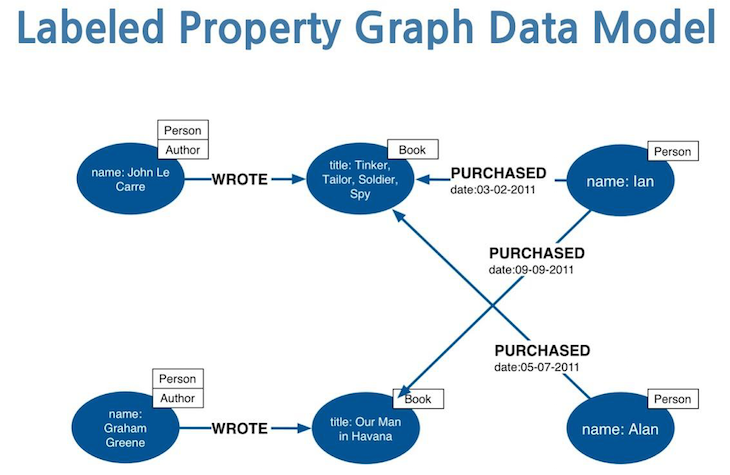
\includegraphics[width=0.75\textwidth]{neo4j}
\caption{The Neo4j model}
\label{fig:neo4j}
\end{figure}

Besides the aforementioned useful properties of Neo4j, we can put the graph to good use for visualising the global urban network. By adding a location property to a city, we can directly map nodes and relations to a geographical map. Most importantly, we can store indices of text files that mention the city as properties of nodes. That way, we are able to generate a subset of files that we can analyse for calculating the strength of the relationship between the nodes.

\subsection{Filtering and Classifying}

\subsubsection{Clustering}
\subsubsection{Filtering}

\subsubsection{Machine Learning for classification}
Text based machine learning can be done in two different ways depending on whether the text is structured or unstructured. Text is structured when sentences are used, meaning grammar is used. In the case of structured texts a word may say something about the next word in the sentence, therefor other techniques can be used (for example n-grams) then in case of unstructured texts.
Machine learning for website classification works by using the raw text from a website. Because the text from websites can be structured as well as unstructured, the unstructured 'bag of words' model is used. This model counts how often each word is used. There are 3 libraries available which contain most steps needed. There is scikit-learn \cite{scikit-learn} and TensorFlow \cite{tensorFlow} for Python and Weka \cite{weka} for Java.
The machine learning works in 4 steps:
\begin{enumerate}
    \item \textbf{Creating a feature extractor} \\
    Given text from a website, the "features" from this text are returned. Features are the words that occur in the text and the number of occurrences. Before this data is extracted stop words (the, is, at etc) are removed and the rest of the words are stemmed meaning all words will be changed to their root-forms (features - feature, controlled - control). The program Snowball \cite{snowball_dutch} and NLKT \cite{nlkt_stemming} (which uses the snowball version) have a dutch implementation for this, although it might need to be improved a bit.
    
    Afterwards, to prepare the features for the machine learning algorithm. We need to give each feature a numeric id. Count each of these tokens. And we need to normalise the tokens. For this scikit-learn provides algorithms.
    \item \textbf{Manually labelling} \\
    For each of the classes (e.g. business, tourism, art etc) we select a few websites we know fit to that class. From these websites all the words will be extracted and their occurrence will be counted. Possibly some normalisation functions are applied to get better values. We call these values the weight for each word for each class. From this we create a two dimensional array with in the rows each of the websites and in the columns all different words and one extra for the class. We fill the fields with the weights or a zero if the words don't occur.
    
    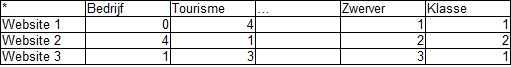
\includegraphics{classTable}
    
    \item \textbf{Generating a classifier} \\
    The array is fed to a learning algorithms. This will generate a classifier. There are a multitude of classifiers importable from Scikit-learn and TensorFlow. For choosing the classifier we make use of the Microsoft Azure Machine Learning Test Sheet \cite{MLCheatSheet}. Several factors should be taken into account when choosing an algorithm. These are:
    \begin{enumerate}
        \item Accuracy - How well the algorithm separates the websites.
        \item Training Time - How long it takes to train the algorithm.
        \item Linearity - Linear regression assumes data trends follow a straight line. This is trade-off between accuracy and speed.
        \item Number of Parameters - Adjustable parameters increase the flexibility of the algorithms. This is a trade-off between training time and accuracy.
        \item Number of Features - A large number of features can make some algorithms unfeasibly long. Especially text data (what we are using!) has a large number features. Support Vector Machines are especially well suited in this case.
        \item Special Cases - Some learning algorithms make particular assumptions about the data or the results.
    \end{enumerate}
    
    For textual data especially support vector machines are recommended, so it is most likely we will choose that machine learning algorithm. Depending on if we have time we might do some tests before making our decision however.
    
    \item \textbf{Entering new examples} \\
    When a new (unlabelled) example (website) comes - extract the features and feed it to your classifier - it will tell you what it thinks it is (and usually - what is the probability the classifier is correct). Afterwards the classifier is updated to include new features extracted from the example.
\end{enumerate}

\subsubsection{TF-IDF}
basic idea: 1. using training data to assign values on words - filter meaningless words - assign words with highest value as categories? 2. Do the same on training data for each category (choose a few documents manually per category) and then check for websites for which categories has the highest value.

\subsection{Search Queries}

\subsubsection{Enter Queries}
\subsubsection{Get Results}
\subsubsection{Specifications}

\subsection{Visualisation}
\todo{Refer to Neo4j graph model \& properties}

\subsubsection{Connection between cities}
\subsubsection{The Strength of these connections}